\section{实验结果}

\subsection{多任务超参数调节}
\label{sec:4_omega}
本章提出的多任务训练方法包含了翻译和CER两个由超参数$\omega$控制训练比例的任务,而CER又包含了TER、VER和TNER三个由$\alpha$、$\beta$和$\gamma$三个超参数控制的子任务。因此如何平衡这些任务的训练比重是在模型训练过程中极为重要的问题。本章根据三个子任务的重要程度,将$\alpha$、$\beta$和$\gamma$三个超参数的比例固定为$2:2:1$,然后通过调节超参数$\omega$来寻找翻译和CER两个任务合适的训练比例。本节依据CER-NMT在英德翻译、英法翻译以及英捷翻译验证集的BLEU值结果来选取一个合适的$\omega$值。

%\begin{figure}[!htbp]
%    \centering
%    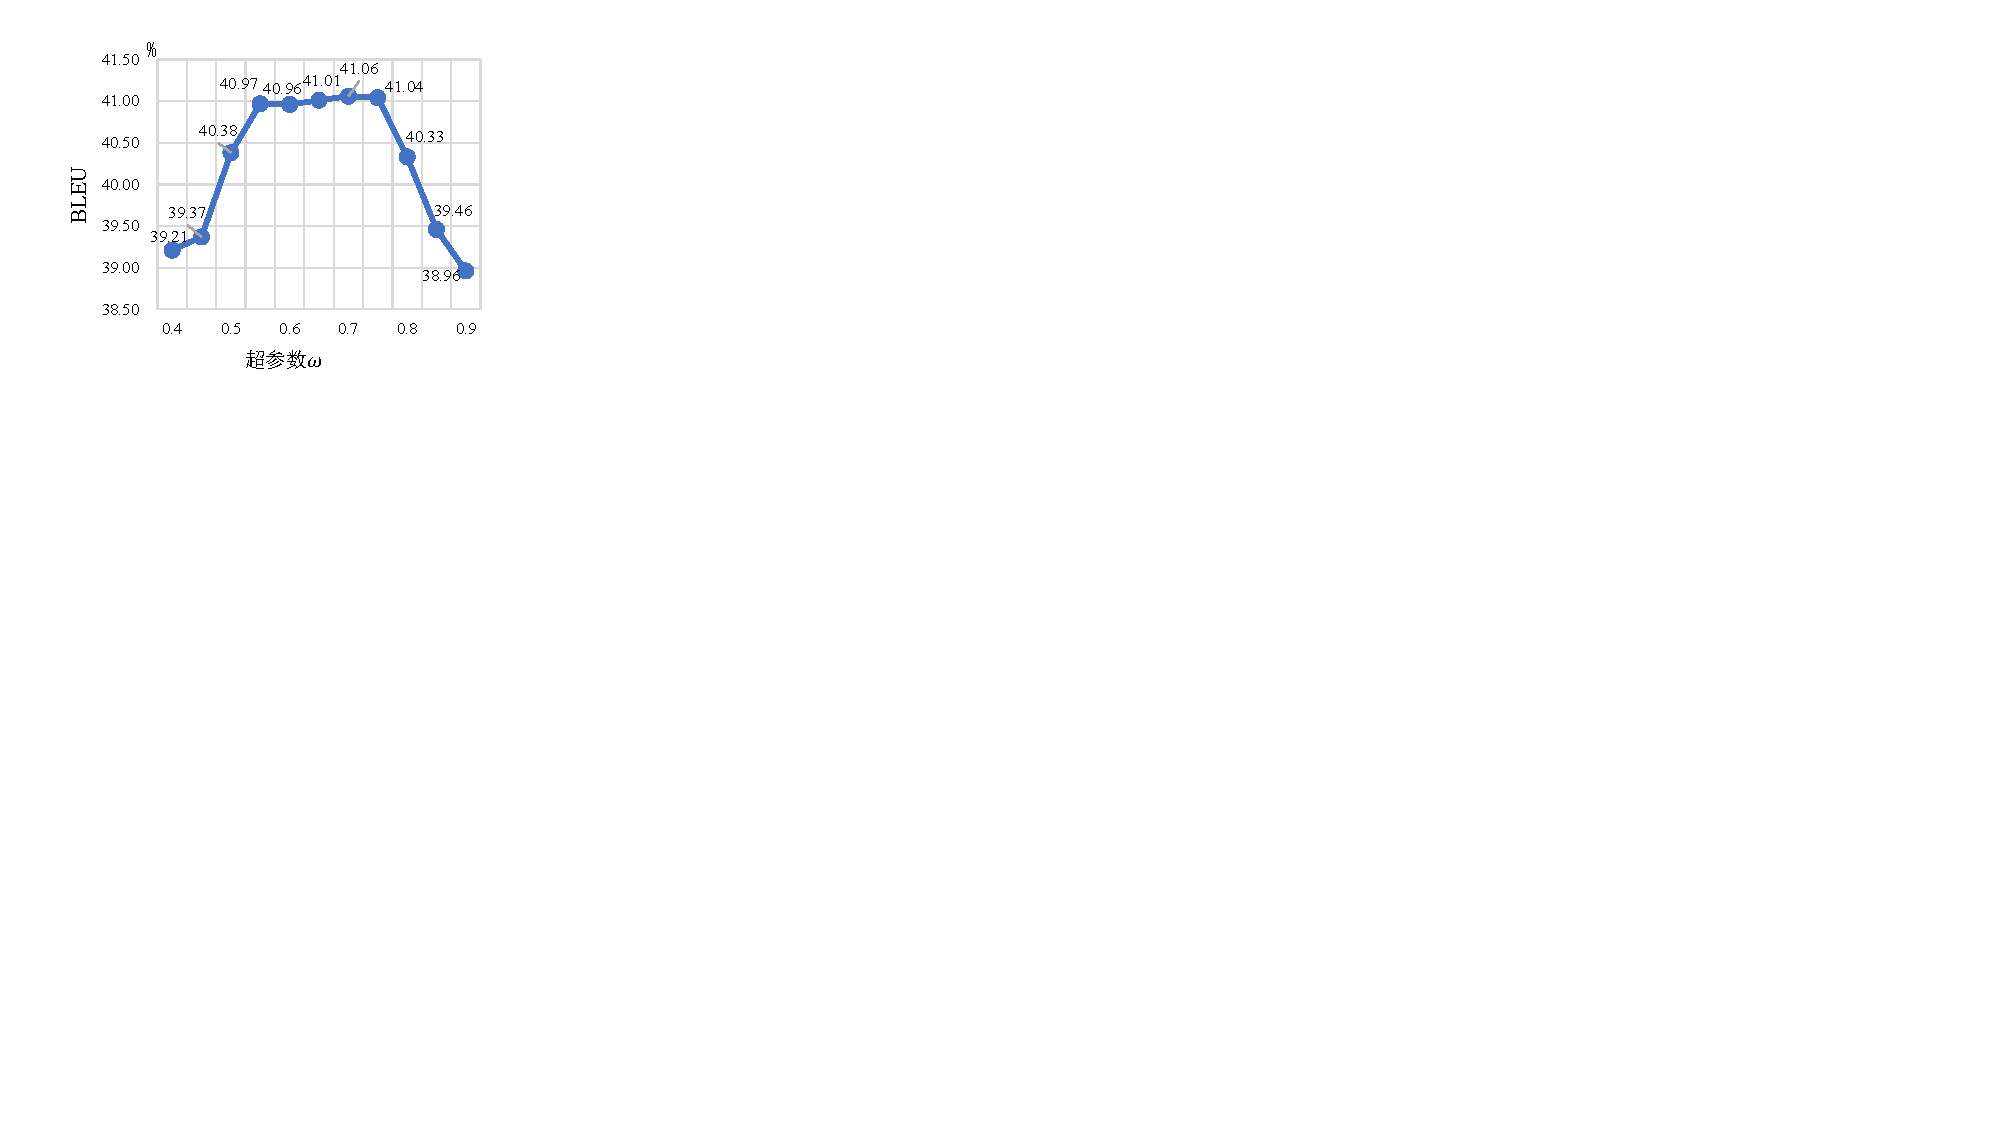
\includegraphics[scale=1.2]{Img/fig_4_searchw.pdf}
%    \bicaption{超参数$\omega$对CER-NMT翻译准确率的影响}{Effect of hyperparameter $\omega$ on translation accuracy of CER-NMT}
%    \label{fig:4_searchw}
%\end{figure}


\begin{figure}[!htbp]
    \centering
    \begin{subfigure}[b]{0.5\textwidth}
      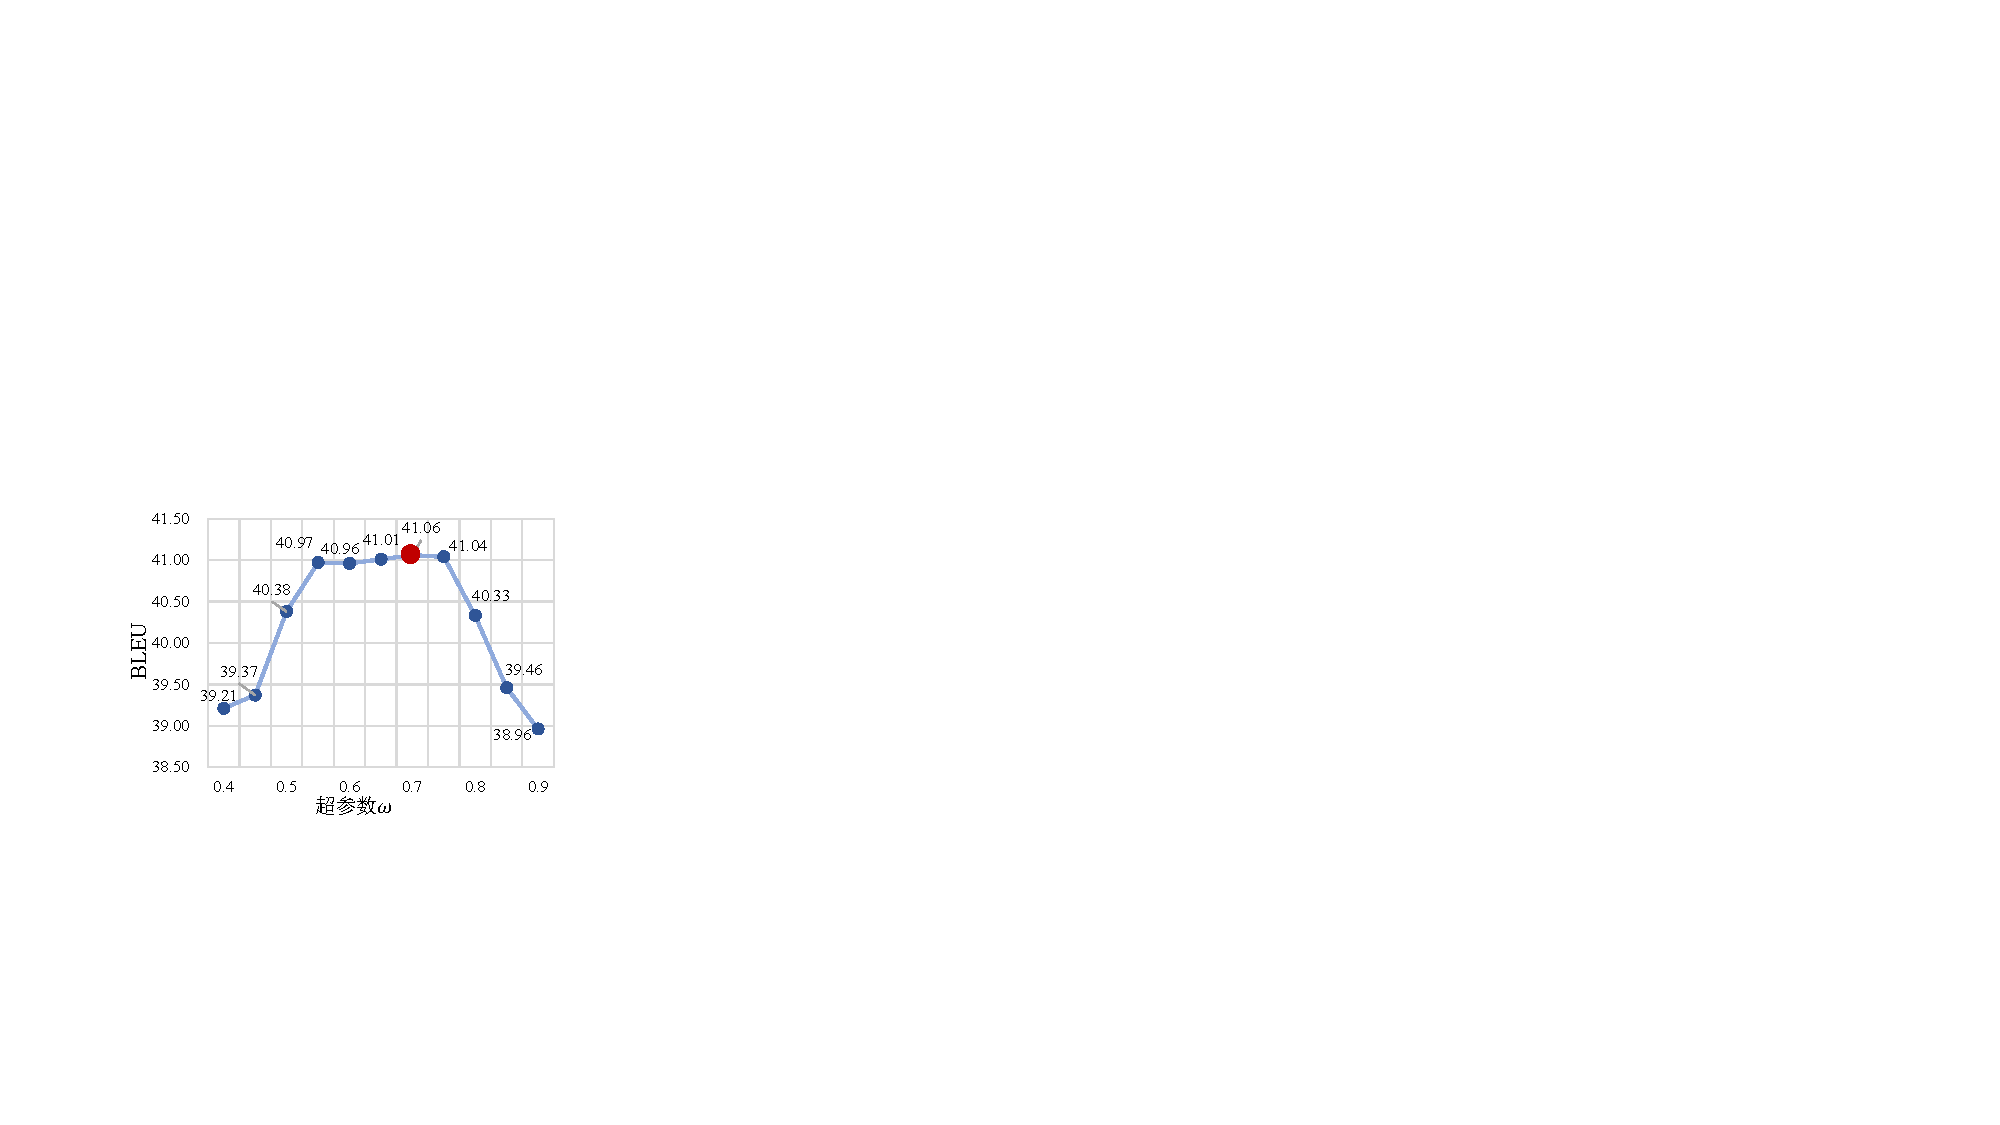
\includegraphics[width=\textwidth]{Img/fig_4_searchw_ende.pdf}
      \caption{英德翻译}
      \label{fig:4_searchw_ende}
    \end{subfigure}%
    ~% add desired spacing
    \begin{subfigure}[b]{0.5\textwidth}
      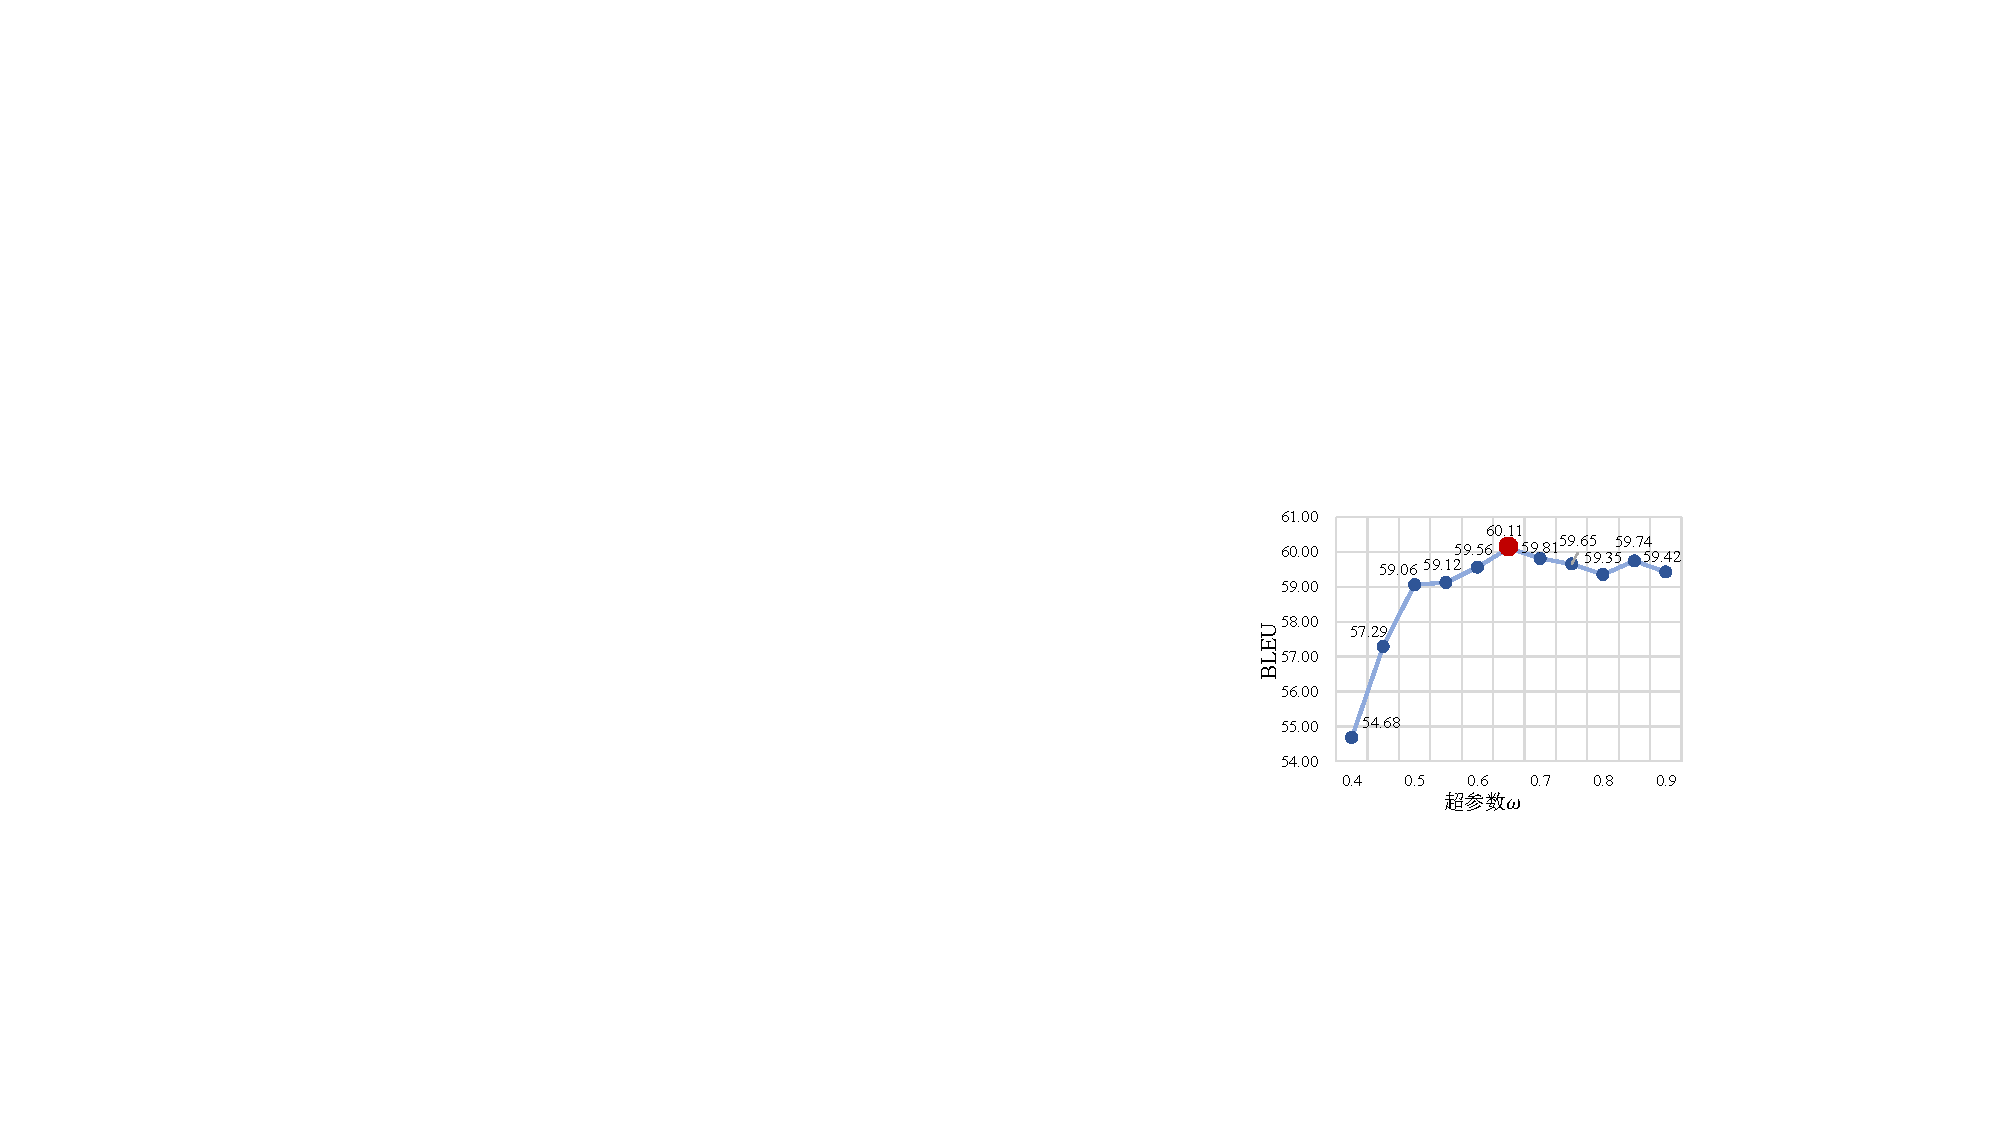
\includegraphics[width=\textwidth]{Img/fig_4_searchw_enfr.pdf}
      \caption{英法翻译}
      \label{fig:4_searchw_enfr}
    \end{subfigure}
    \\% line break
    \begin{subfigure}[b]{0.5\textwidth}
      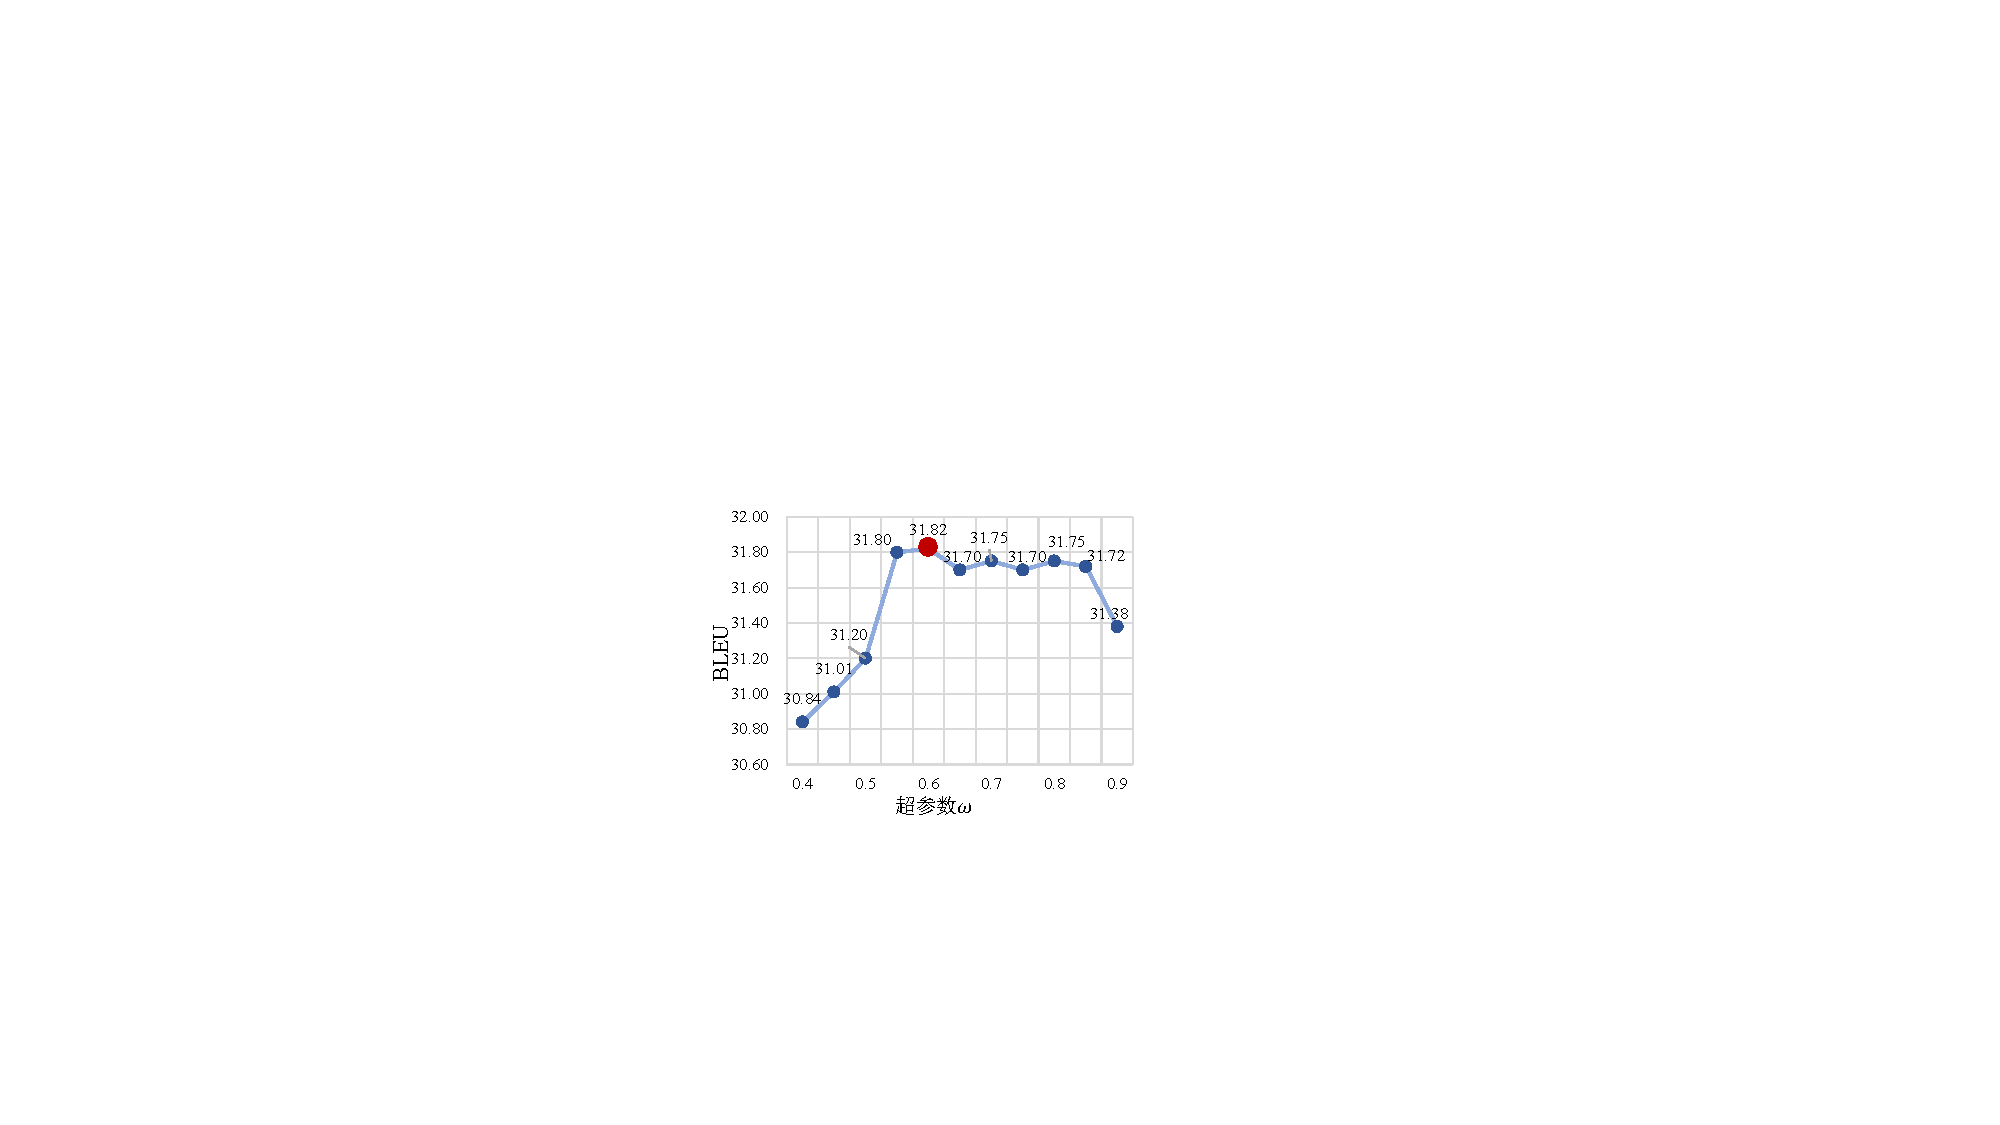
\includegraphics[width=\textwidth]{Img/fig_4_searchw_encs.pdf}
      \caption{英捷翻译}
      \label{fig:4_searchw_encs}
    \end{subfigure}%
    \bicaption{超参数$\omega$对CER-NMT翻译准确率的影响}{Effect of hyperparameter $\omega$ on translation accuracy of CER-NMT}
    \label{fig:4_searchw}
\end{figure}
如图\ref{fig:4_searchw}所示实验结果,横轴代表$\omega$从0.4以0.05为间隔增加至0.9,纵轴为NMT模型在英译德验证集上的BLEU值。当$\omega=1.0$时,代表翻译任务的训练比例为$100\%$,此时是纯文本神经机器翻译。当$\omega=0.0$时,代表仅训练CER不做翻译。该图反映出,当$\omega \in [0.55,0.8]$时,模型普遍具有较好的BLEU值结果。超过这个范围时,CER-NMT的BLEU值将逐渐接近纯文本翻译模型。低于这个范围时,CER-NMT的翻译准确率发生了骤减。我们还测试了当$\omega=0.3$时的情况,此时英德翻译的BLEU值以骤减到9.86,英法骤减到8.62,英捷翻译骤减到3.94。以上实验结果说明在一个合适的范围内,CER方法能够帮助翻译模型提升翻译准确率。而这个范围应当使模型的训练过程主要以翻译任务为主以CER为辅。因此,本章选择$\omega=0.7$作为英德翻译模型的超参数,$\omega=0.65$作为英法翻译模型的超参数,$\omega=0.6$作为英捷翻译模型的超参数,即CER-NMT在验证集上达到最高的BLEU值时,作为后续试验中对超参数$\omega$的设置。


\subsection{翻译结果}
\label{sec:4_translation_results}


\begin{table}[!htbp]
    \bicaption{在Multi30K英德翻译、英法翻译和英捷翻译上的结果。}{Translation results on Multi30K EN-DE, EN-FR, EN-CS.}
    \label{tab:4_ende_enfr_encs}
    \centering
    \footnotesize% fontsize
    \setlength{\tabcolsep}{4pt}% column separation
    \renewcommand{\arraystretch}{1.2}%row space 
\begin{tabular}{ccccccccccc}
\hline
 \multirow{3}{*}{模型} & \multicolumn{6}{c}{英德翻译} & \multicolumn{2}{c}{英法翻译} & \multicolumn{2}{c}{英捷翻译} \\
\cmidrule(r){2-7} \cmidrule(r){8-9} \cmidrule(r){10-11}%\hline
       & \multicolumn{2}{c}{Test2016} & \multicolumn{2}{c}{Test2017} & \multicolumn{2}{c}{MSCOCO} & \multicolumn{2}{c}{Test2016} & \multicolumn{2}{c}{Test2016} \\
\cline{2-11}%\cmidrule(r){2-7} \cmidrule(r){8-9} %\cline{2-9}
              &    BLEU & Meteor &     BLEU & Meteor &     BLEU & Meteor &     BLEU & Meteor  &   BLEU & Meteor \\
\hline
\multicolumn{11}{c}{图片信息辅助式方法} \\
\hline
SerialAtt\pcite{libovicky2018input}      & 38.7 & 57.2 & - & - & - & - & 60.8 & 75.1 & 31.0 & 29.9 \\
DelMMT\pcite{ive2019distilling}           & 38.0 & 55.6 & - & - & - & - & 59.8 & 74.4 & - & -\\
GAMMT\pcite{liu2021gumbel}      & 39.2 & {\textbf{57.8}} & 31.4 & 51.2 & 26.9 & 46.0 & - & - & - & -\\
GMMT\pcite{yin2020novel}             & 39.8 & 57.6 & 32.2 & 51.9 & 28.7 & {\textbf{47.6}} & 60.9 & 74.9 & - & -\\
\hline
\multicolumn{11}{c}{图片信息增强式方法} \\
\hline
Imagination\pcite{elliott2017imagination}      & 36.8 & 55.8 & - & - & - & - & - & - & - & -\\
ImagiT\pcite{long2021generative}   & 38.6 & 55.7 & 32.1 & {\textbf{52.4}} & - & - & 59.9 & 74.3 & - & -\\
CTR-NMT             & 39.7 & 57.5 & {\textbf{32.9}} & 51.7 & {\textbf{29.1}} & 47.5 & 61.1 & 75.8 & 32.7 & 30.7\\
\hline
\multicolumn{11}{c}{本章所提方法} \\
\hline
Transformer\pcite{vaswani2017attention}             & 38.5 & 57.5 & 31.0 & 51.9 & 27.5 & 47.4 & 60.5 & 75.6 & 30.8 & 29.8 \\
CER-NMT          & {\textbf{40.2}} & {\textbf{57.8}} & 32.5 & 52.0 & 28.3 & 47.1 & {\textbf{61.9}} & {\textbf{76.4}} & {\textbf{32.9}} & {\textbf{31.2}}\\
\bottomrule
\end{tabular}
\end{table}

表\ref{tab:4_ende_enfr_encs}显示了采用了CER方法的神经机器翻译系统的翻译结果。其中$\omega$按照4.1节的结论,针对英德翻译、英法翻译和英捷翻译的取值分别为0.7、0.65和0.6。对于VER、TER和TNER三个子任务,$\alpha$、$\beta$和$\gamma$的值分别设置为0.4、0.4和0.2。


表\ref{tab:4_ende_enfr_encs}中加粗项表示整列中的最佳结果。根据以上英德翻译、英法翻译和英捷翻译的实验结果可以得到以下结论:

%\begin{itemize}
%\item
(1)本章所提方法在Multi30K Test2016测试集的英德翻译、英法翻译和英捷翻译三个翻译对上取得了BLEU和Meteor值的最佳结果,并且在英德翻译Test2017测试集上的结果超过了多数模型的结果,并与其它模型的最佳结果相比差距很小。这说明CER方法能够有效提升NMT模型的翻译质量。

%\item
(2)CER-NMT在歧义词较多的Ambiguous MSCOCO上的表现并不理想,落后于GMMT和上一章的CTR-NMT两个模型。这是因为CER方法主要帮助翻译模型在训练阶段融合视觉信息,在测试阶段因为不需要输入图像使得模型无法借助视觉信息解决歧义词的问题。同理可以看到,CTR-NMT在Meteor上的提升也仅有0.1。这说明图片信息增强式的方法虽然能够提升模型的翻译质量,但也同样具有一定的局限性。例如文本中常见的歧义词问题或语义不完整问题,是需要利用图片信息辅助翻译模型来解决。

(3)%\item
GMMT、CTR-NMT和CER-NMT均是采用视觉目标作为视觉输入的方法,其结果均优于采用完整图片输入的方法。理想的情况下,完整的图片包含的视觉信息更完整,对翻译带来的好处会更多。但是目前实验结果说明,在神经机器翻译中融合图片信息是非常困难的,需要为NMT模型提供更细粒度的视觉信息才能降低跨模态信息融合的难度,从而使模型更多地利用图片中的视觉信息。
%\end{itemize}

综合以上的实验结果,本章所提的跨模态实体重构方法能有效地提升机器翻译的质量。同时也说明了虽然图片信息增强式的翻译方法无法解决歧义词及语义不完整等问题,但是方法的有效性也体现了图片信息具有除补全语义以外的其它作用。

\subsection{消融实验}
\label{sec:4_ablation_study}
为了探究VER、TER和TNER三个子任务对CER$-$NMT模型的影响,本节设置了12组消融实验。其中序号0代表\ref{sec:4_translation_results}节中CER-NMT的结果。序号1$-$3组各去掉一个子任务,并保持剩余子任务的训练权重。序号4$-$5组各去掉一个子任务,保持NMT的权重。序号7$-$9组各保留一个子任务,保持子任务的权重。序号10$-$12组保留一个子任务,保持NMT的权重。

\begin{table}[!htbp]
    \bicaption{在Multi30K Test2016英德翻译上消融实验结果}{Ablation study results on the EN-DE of Multi30K Test2016}
    \label{tab:4_ablation_study}
    \centering
    \footnotesize% fontsize
    \setlength{\tabcolsep}{4pt}% column separation
    \renewcommand{\arraystretch}{1.2}%row space 
\begin{tabular}{cccccc}
\hline
\multirow{2}{*}{序号} & NMT & VER & TER & TNER & \multirow{2}{*}{BLEU} \\
\cline{2-5}
   & $\omega$ & $(1-\omega) \times \alpha$ & $(1-\omega) \times \beta$ & $(1-\omega) \times \gamma$ & \\
\hline
0  & 0.70 & 0.12 & 0.12 & 0.06 & 40.2 \\
\hline
1  & 0.76 & 0.12 & 0.12 &  -   & 40.0 \\
2  & 0.82 & 0.12 & -    & 0.06 & 39.5 \\
3  & 0.82 & -    & 0.12 & 0.06 & 39.6 \\
\hline
4  & 0.70 & 0.15 & 0.15 & -    & 39.9 \\
5  & 0.70 & 0.20 & -    & 0.10 & 39.2 \\
6  & 0.70 & -    & 0.20 & 0.10 & 39.3 \\
\hline
7  & 0.88 & 0.12 & -    & -    & 38.8 \\
8  & 0.88 & -    & 0.12 & -    & 38.8 \\
9  & 0.94 & -    & -    & 0.06 & 39.0 \\
\hline
10 & 0.70 & 0.30 & -    & -    & 39.2 \\
11 & 0.70 & -    & 0.30 & -    & 39.4 \\
12 & 0.70 & -    & -    & 0.30 & 39.0 \\
\hline
\end{tabular}
\end{table}

实验结果如表2所示,其中“-”代表所对应的子任务被去掉,可以获得如下信息:

%\begin{itemize}
%\item
(1)序号1$-$6组各去掉了一个子任务,序号7$-$12组各仅保留一个子任务。从两组之间的对比可以看出,1$-$3的结果整体优于7$-$8,4$-$6的结果整体优于10$-$12,说明无论是保持子任务的训练比重不变还是保持翻译任务的训练比重不变,子任务组合的方式总是优于仅使用单一的子任务。其中,VER和TER的在序号1和4中的组合已经可以使翻译模型得到很好的结果。TNER对NMT的影响最小,但是依旧可以为NMT模型带来小幅度的提升。

%\item
(2)$\omega>0.8$的实验组2,3,7,8,9的结果与\ref{sec:4_omega}小节中的实验结果均说明减少跨模态任务至一定比重后,模型结果的BLEU值将逐渐趋近于纯文本翻译模型。因此在多任务训练阶段,不能因为翻译时主任务就将CER的比例调节的过低,保持两者的平衡更重要。

%\item
(3)与\ref{sec:4_translation_results}小节中CER-NMT的实验结果相比可以说明,针对实体重构的VER和TER任务对翻译模型的性能影响最大,且这两个任务组合情况下的结果要优于单独使用的情况。相比之下,TNER同样可以为翻译性能带来一定的提升,但效果不如实体重构明显。综合以上,TER、VER和TNER三个子任务共同配合可以使翻译模型的性能达到最佳。
%\end{itemize}

消融实验的结果说明了本章所提的双向实体重构方法是有效的,视觉实体重构能够帮助文本实体重构进一步提升模型的翻译质量。文本非实体重构虽然为模型的性能提升带来的效果相对较小,但是将其与双向实体重构组合到一起可以得到CER方法的最佳效果。

\subsection{文本实体忠实度}
\label{sec:4_fidelity}
本章所提方法对视觉实体与文本实体互相结合跨模态信息,再将视觉实体与文本上下文相融合。而这一过程中是以实体间的信息融合为主导的,\ref{sec:4_ablation_study}小节的实验也证实了这一点。这使得视觉信息具有明确的作用方向。因此检验视觉信息是否对文本实体的翻译产生了影响成为了一个必要的环节。本节我们将尝试测量模型在解码生成目标单词时对源语言文本实体的忠实度来反映模型的行为变化。


Transformer的解码器采用的是交叉注意力机制,与一般的注意力机制类似的是,在解码过程中通过给源端的词不同的“权重”来达到“关注”或“忽视”的作用。该“权重”体现了当前要解码的目标端单词对源端单词所提供信息的需求程度。因此,我们选择Transformer解码器最后一层交叉注意力权重的多头平均值,作为生成目标端词时对源端词的注意力“权重”,并定义该“权重”为忠实度(fidelity),用于量化生成目标端文本实体时对源端文本实体的忠实程度。\ref{sec:4_dataset}小节中提到,源端的文本实体是通过文本分析工具提取得到。本节中所要确定的目标端文本实体是通过fast-align\cite{45_dyer-etal-2013-simple}对齐工具对齐源端与目标端单词得到的。为了得到一个较好的对齐结果,我们将测试集与训练集拼接后训练对齐模型。

实验结果如图\ref{fig:4_fidelity}所示,图中横轴代表测试集中源语言文本实体以某种方式的排序,纵轴为范围从0到1的忠实度。每个小像素点代表一个源端文本实体在一个翻译句子样本中对应目标端文本实体的注意力权重值,即实体词忠实度。大圆点代表每个实体词的平均忠实度。图\ref{fig:4_fidelity_base}为纯文本Transformer的测试结果,横轴为测试集中的1110个源端文本实体按照平均忠实度由小到大排序。图\ref{fig:4_fidelity_cer_baseorder}为CER-NMT与图\ref{fig:4_fidelity_base}横轴词序保持一致的结果,图\ref{fig:4_fidelity_cer_selforder}为CER-NMT对实体词重排序后的结果。图\ref{fig:4_fidelity_tner}为\ref{sec:4_ablation_study}节序号12仅设置TNER,且保持翻译任务训练比例为70\%不变的模型。图中“avg”代表平均值。从4个图的对比中可以得到以下信息:

%\item
(1)图中忠实度为0的横线部分代表对齐模型无法在目标端句子中找到对应的实体词。因此这些词的忠实度为0。

%\item
(2)图\ref{fig:4_fidelity_cer_baseorder}相比于图\ref{fig:4_fidelity_base}存在更多靠近1.0的小像素点。从图\ref{fig:4_fidelity_cer_selforder}中的均值结果(avg)可以看到,小像素点的均值从0.4238提升至0.4498,大圆点的均值从0.4024提升至0.4478,均具有较明显的提升。该数值结果表明CER方法能够明显地提升模型在翻译过程中对源语言文本实体的忠实度。


\begin{figure}[!htbp]
    \centering
    \begin{subfigure}[b]{0.5\textwidth}
      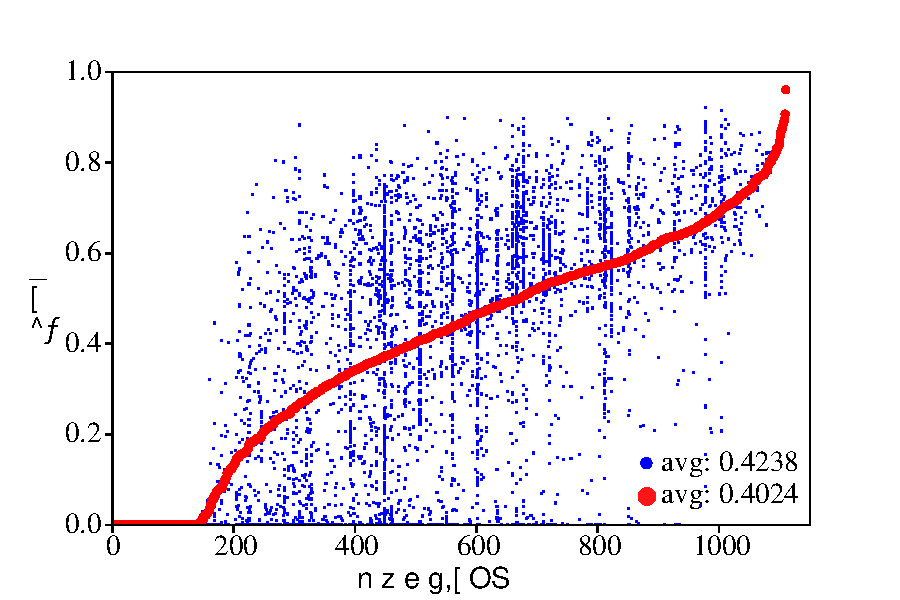
\includegraphics[width=\textwidth]{Img/fig_4_fidelity_base.pdf}
      \caption{Transformer}
      \label{fig:4_fidelity_base}
    \end{subfigure}%
    ~% add desired spacing
    \begin{subfigure}[b]{0.5\textwidth}
      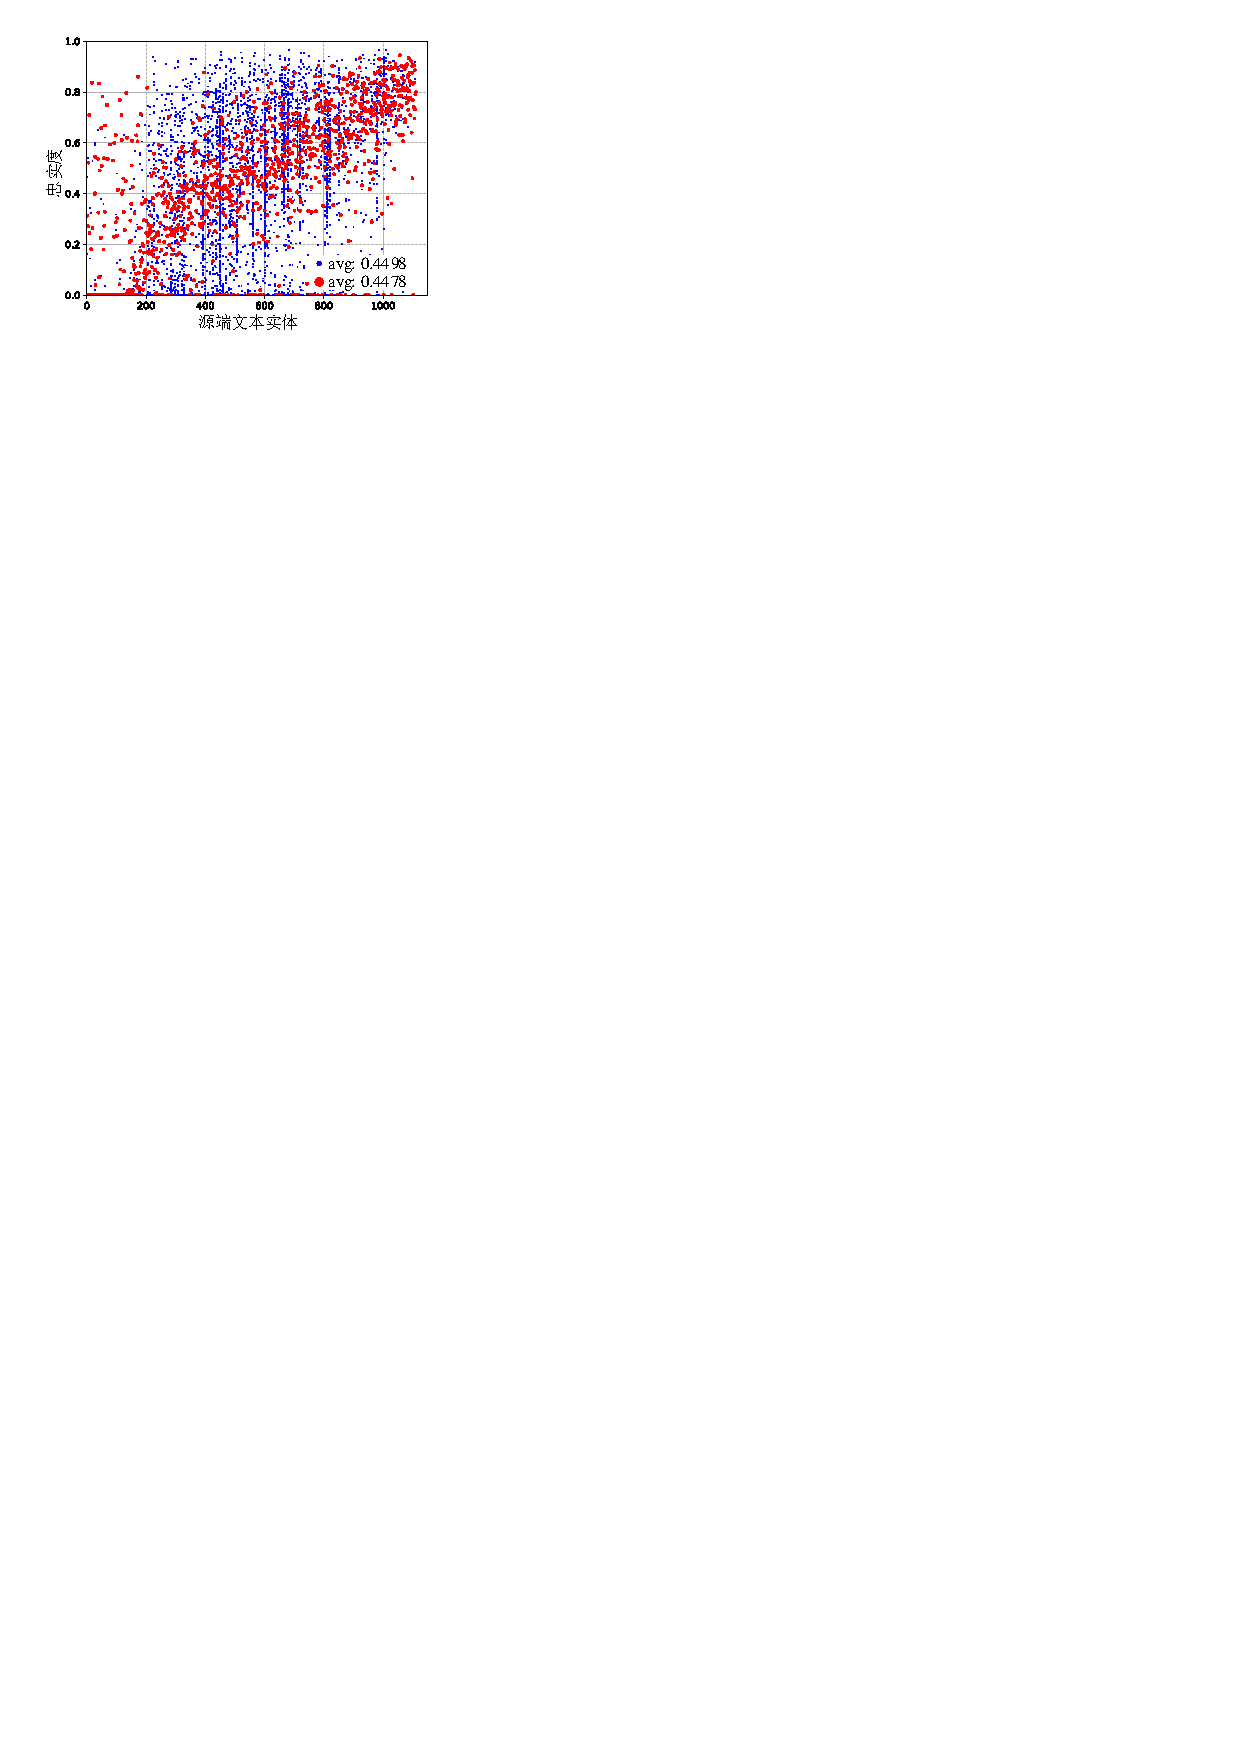
\includegraphics[width=\textwidth]{Img/fig_4_fidelity_cer_baseorder.pdf}
      \caption{CER-NMT}
      \label{fig:4_fidelity_cer_baseorder}
    \end{subfigure}
    \\% line break
    \begin{subfigure}[b]{0.5\textwidth}
      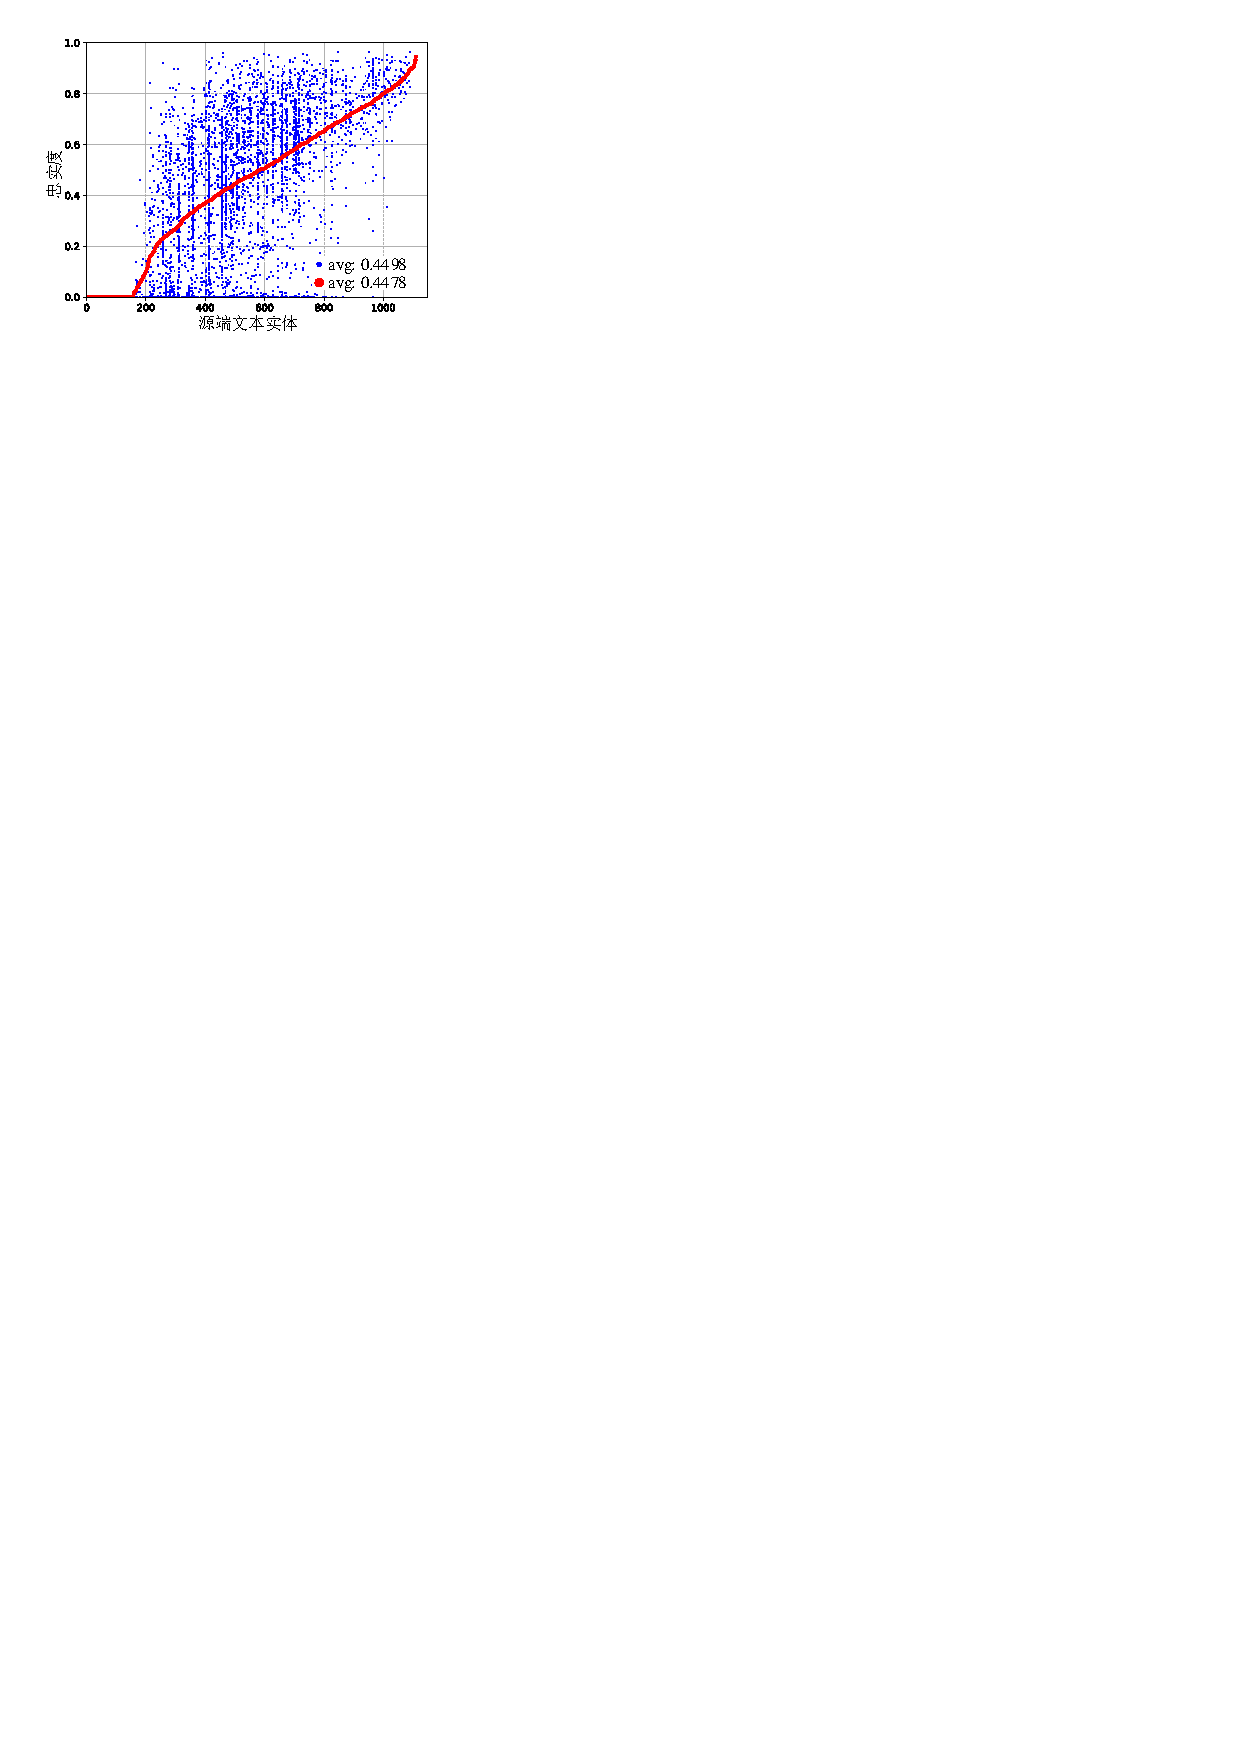
\includegraphics[width=\textwidth]{Img/fig_4_fidelity_cer_selforder.pdf}
      \caption{实体重排序的CER-NMT}
      \label{fig:4_fidelity_cer_selforder}
    \end{subfigure}%
    ~% add desired spacing
    \begin{subfigure}[b]{0.5\textwidth}
      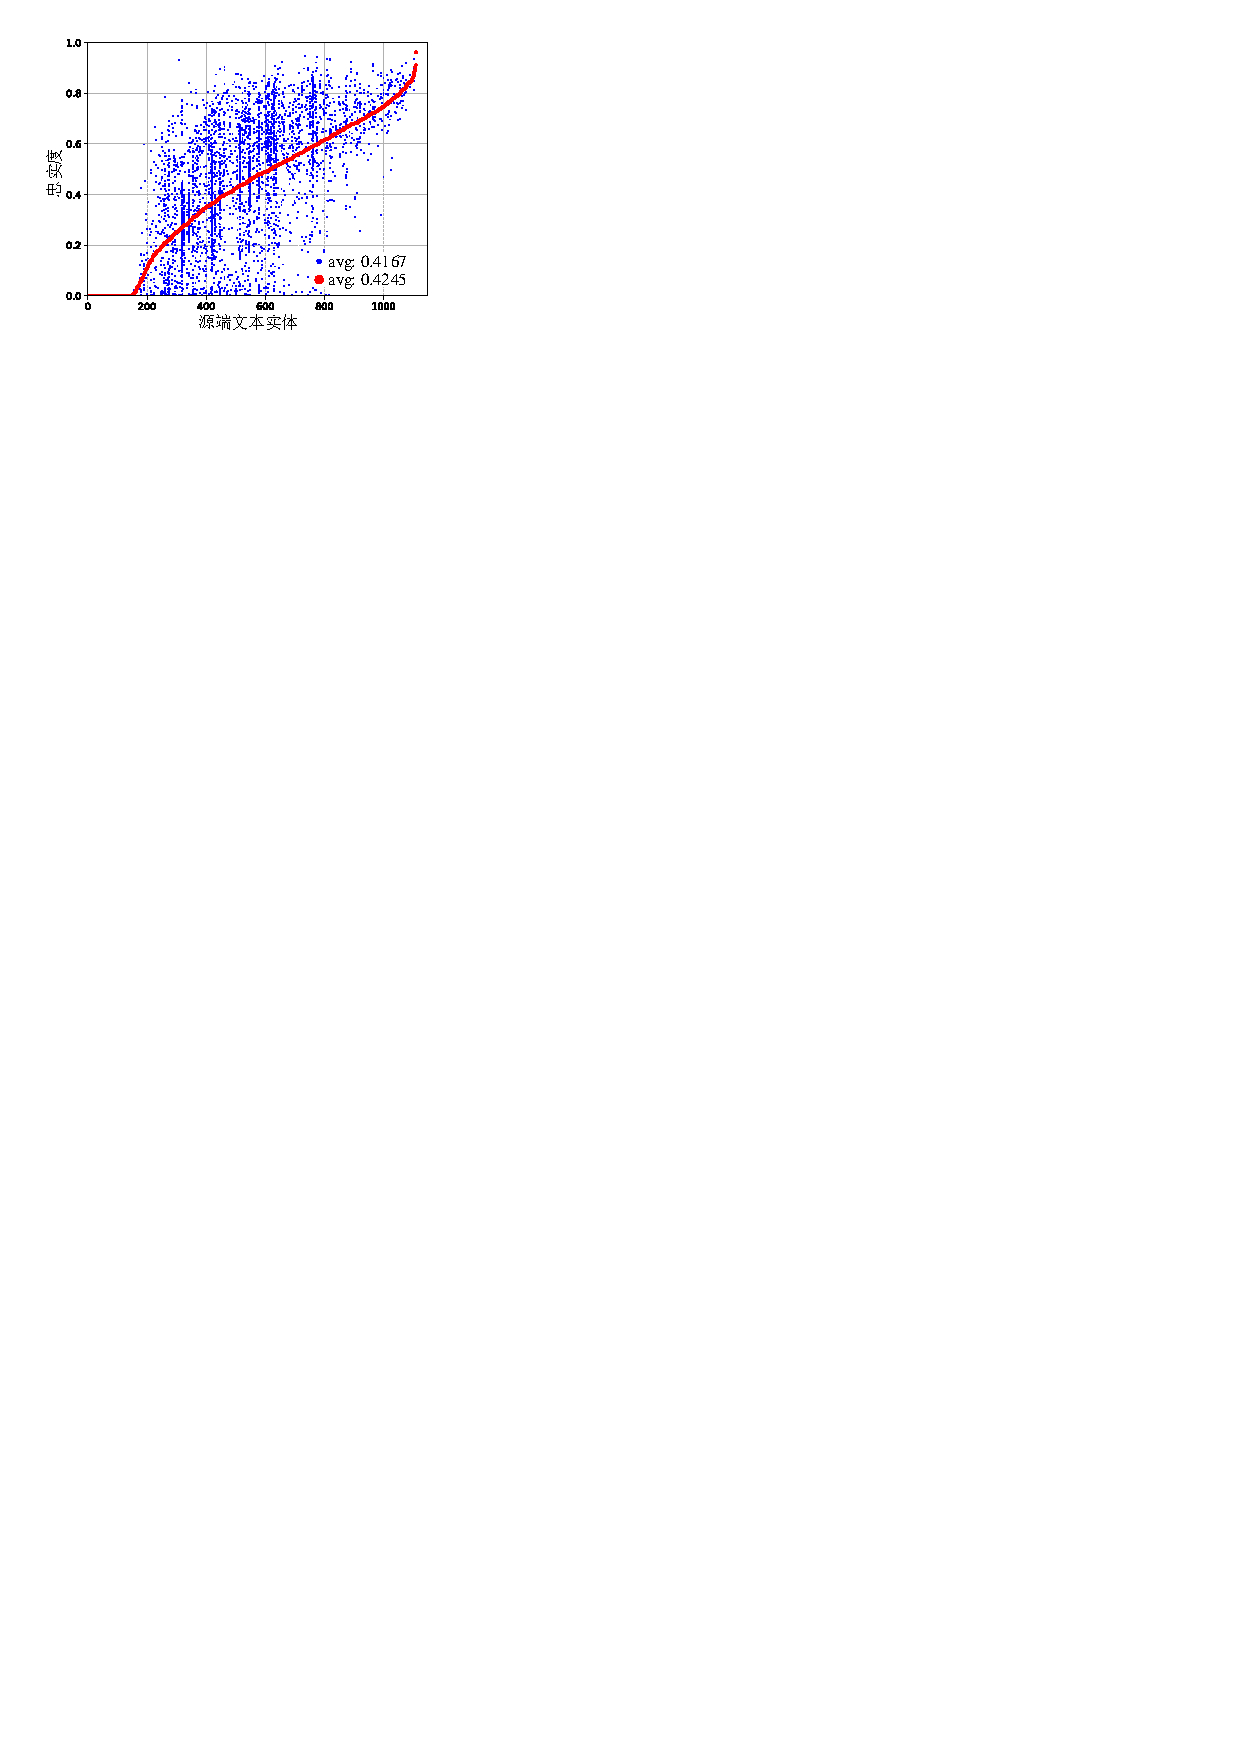
\includegraphics[width=\textwidth]{Img/fig_4_fidelity_tner.pdf}
      \caption{TNER-NMT}
      \label{fig:4_fidelity_tner}
    \end{subfigure}
    \bicaption{文本实体在不同模型下的忠实度}{The fidelity of textual entities on different models}
    \label{fig:4_fidelity}
\end{figure}
%\item
(3)图\ref{fig:4_fidelity_cer_selforder}经过重排序实体的顺序后可以更直观地从曲线的趋势看出采用CER方法所带来的忠实度的提升。

%\item
(4)TNER对文本上下文和视觉实体进行句子级的语义融合,可以观察到图\ref{fig:4_fidelity_tner}相对于图\ref{fig:4_fidelity_base}有提升也有降低,这说明VER和TER才是帮助提升文本实体忠实度的主要因素,针对非实体的重构方法所带来的翻译性能提升无法没有显著地体现在实体忠实度的提升上。
%\end{itemize}

以上结果表明,CER方法通过融入视觉信息的方式,增加了翻译模型在翻译过程中对源语言文本实体的忠实度,从而使得翻译结果得到了进一步的提升。该实验同样表明本章的双向跨模态实体重构方法是有效可行的,该显式跨模态信息融合方法使得模型更具备可解释性,视觉信息的作用方式更有迹可循。

\subsection{基于词频的翻译准确率统计}
\label{sec:4_freq_acc}


\begin{figure}[!htbp]
    \centering
    \begin{subfigure}[b]{0.5\textwidth}
      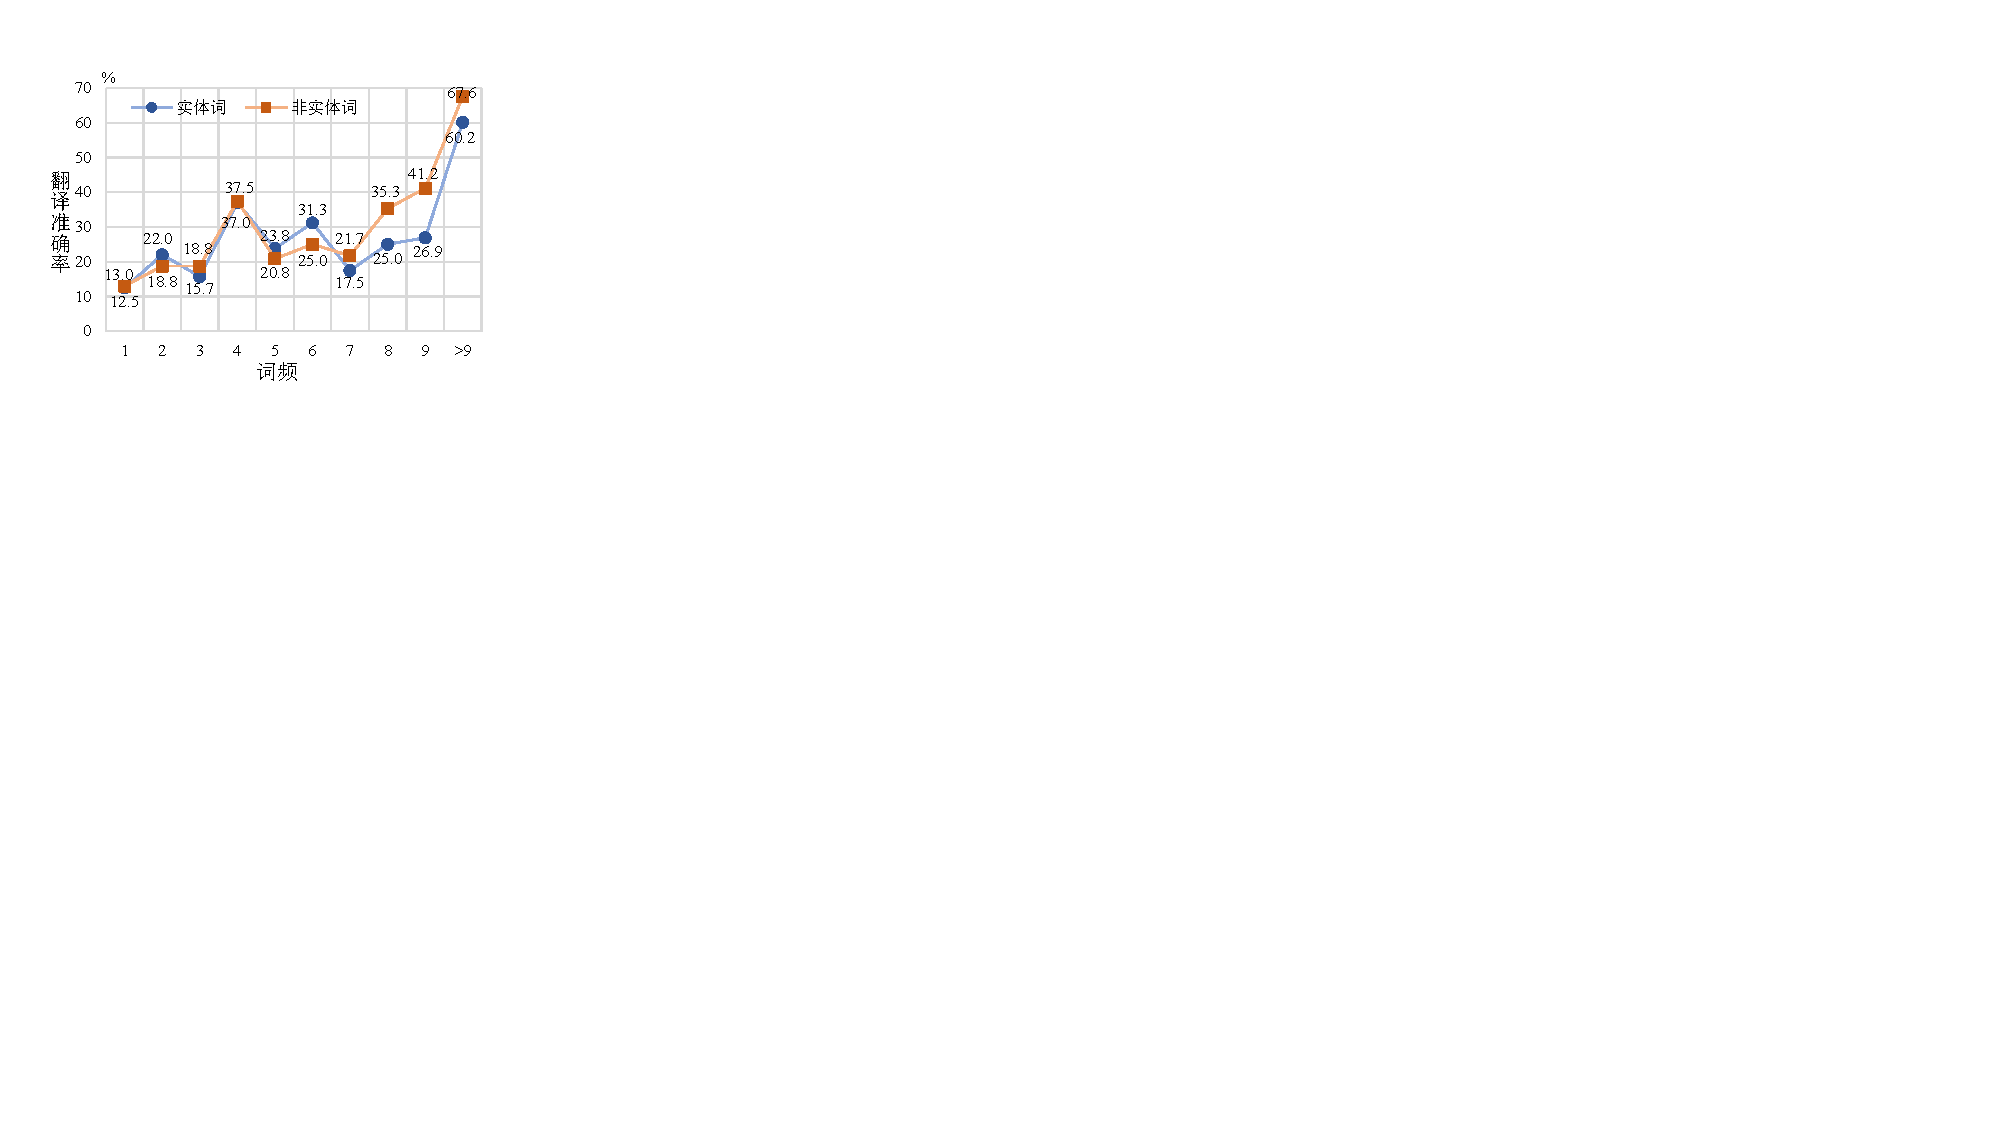
\includegraphics[width=\textwidth]{Img/fig_4_freq_acc_transformer.pdf}
      \caption{Transformer}
      \label{fig:4_freq_acc_transformer}
    \end{subfigure}%
    ~% add desired spacing
    \begin{subfigure}[b]{0.5\textwidth}
      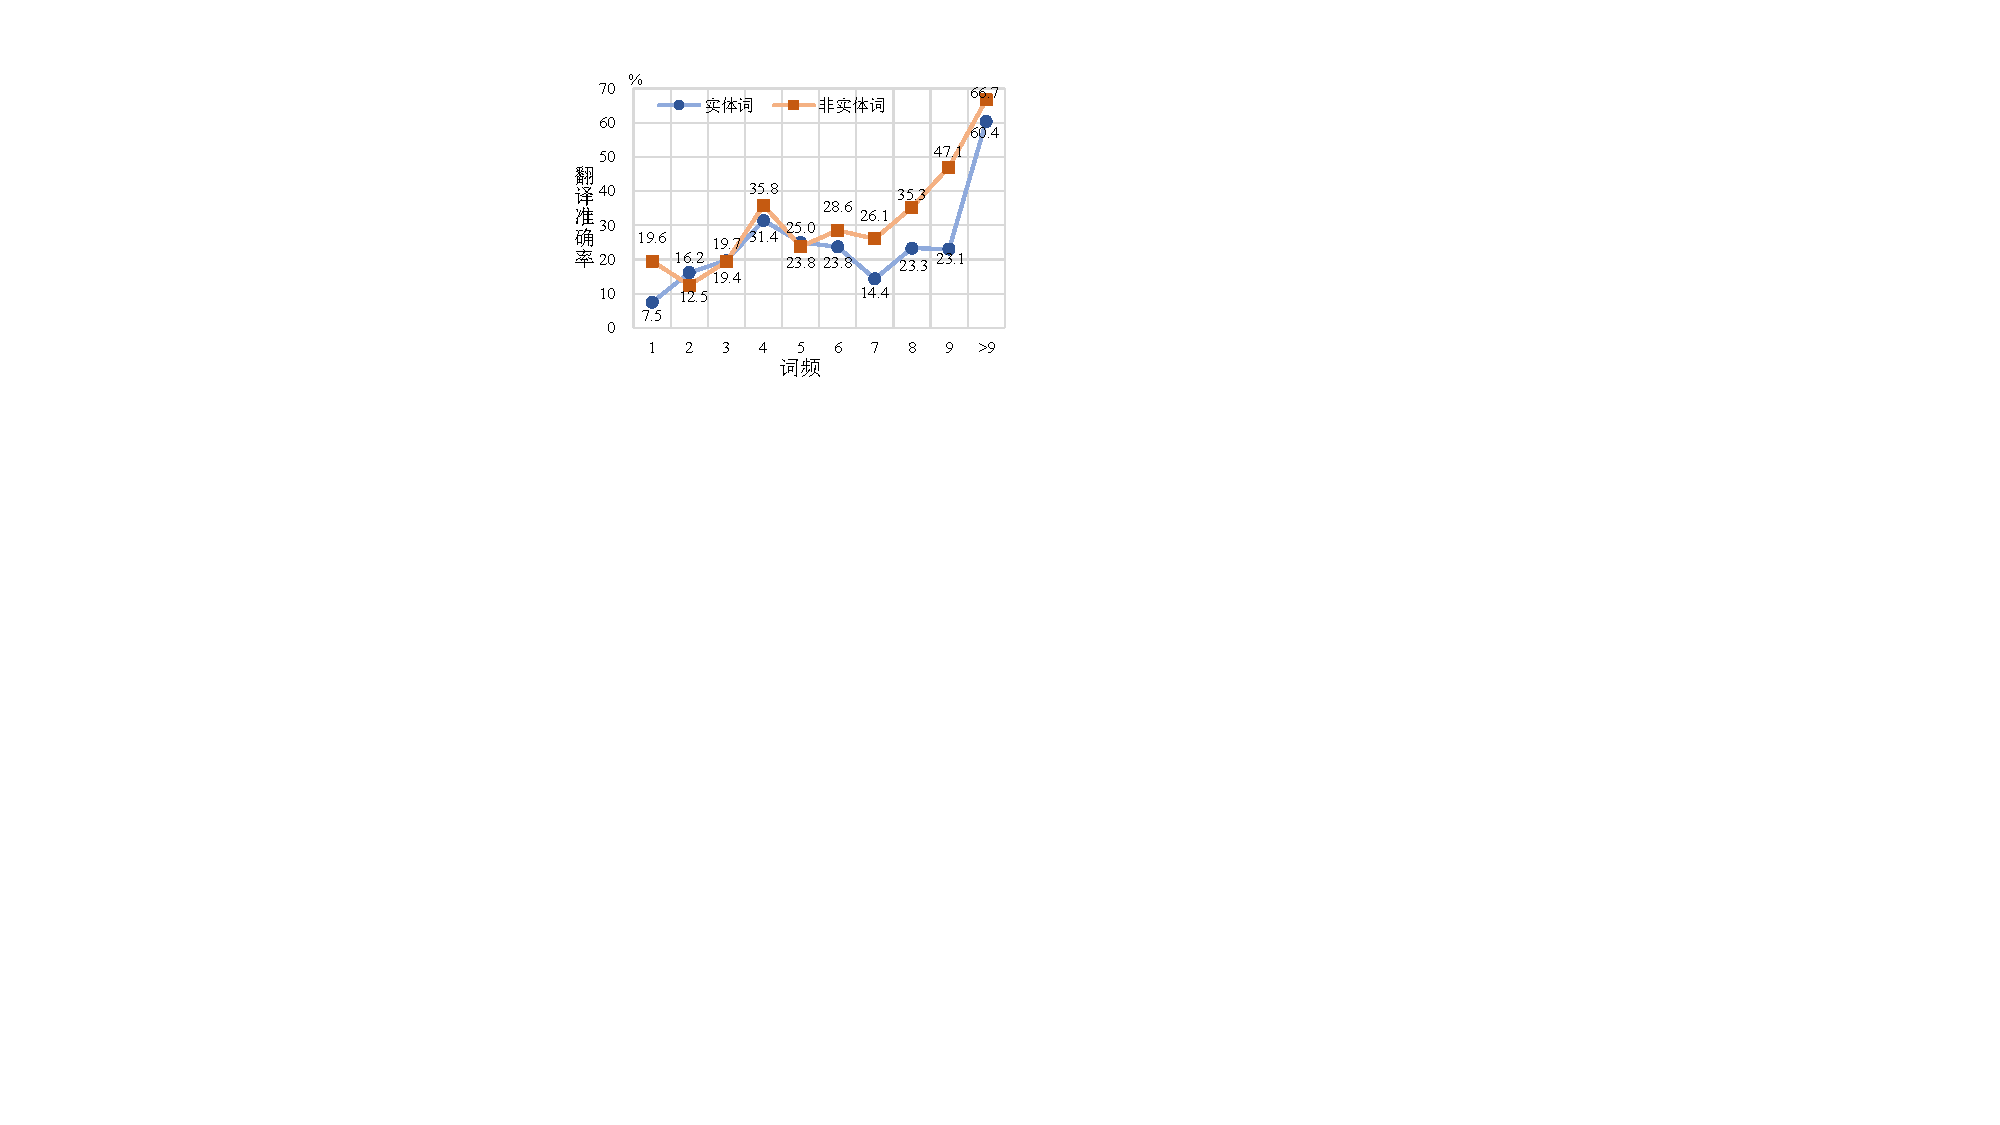
\includegraphics[width=\textwidth]{Img/fig_4_freq_acc_tner.pdf}
      \caption{TNER-NMT}
      \label{fig:4_freq_acc_tner}
    \end{subfigure}
    \\% line break
    \begin{subfigure}[b]{0.5\textwidth}
      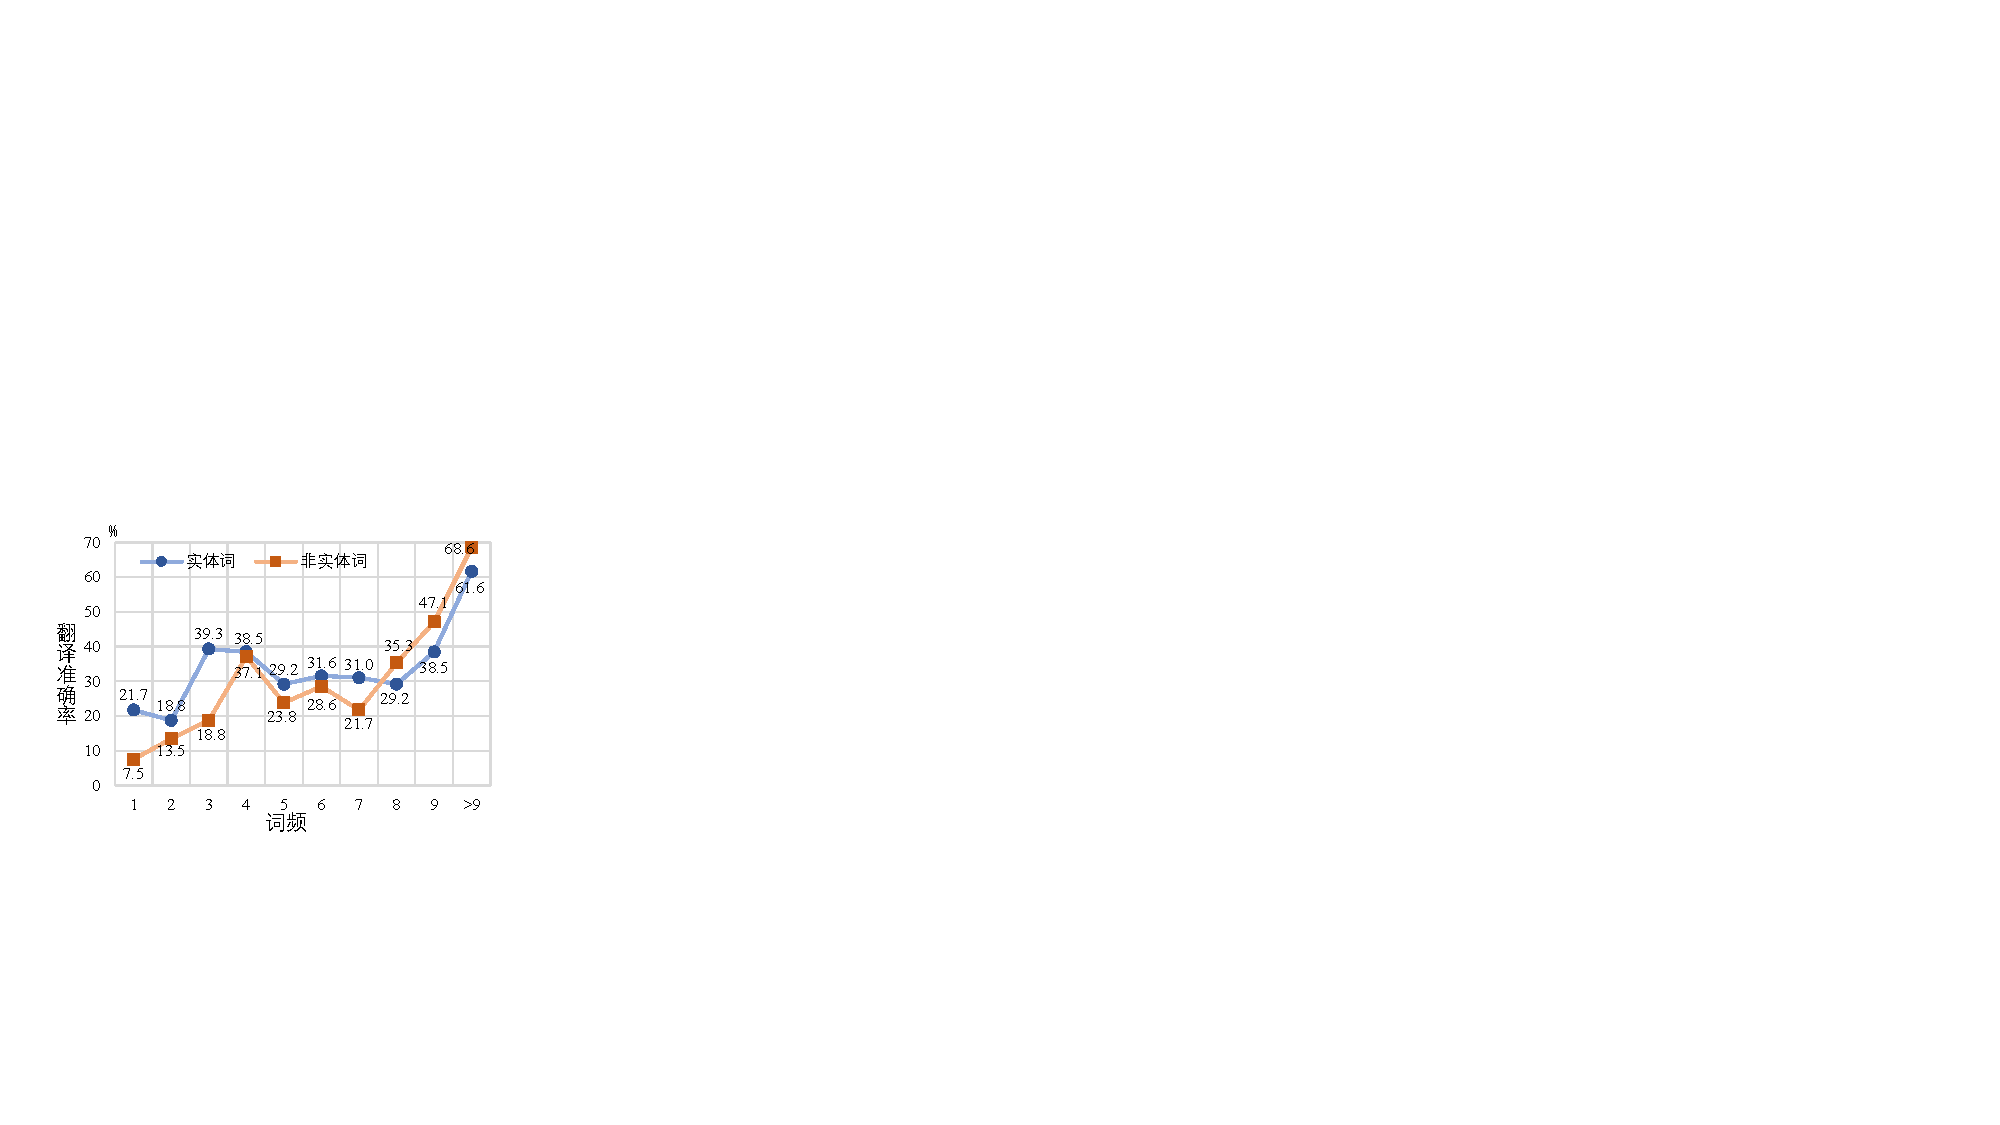
\includegraphics[width=\textwidth]{Img/fig_4_freq_acc_cer.pdf}
      \caption{CER-NMT}
      \label{fig:4_freq_acc_cer}
    \end{subfigure}%
    ~% add desired spacing
    \begin{subfigure}[b]{0.5\textwidth}
      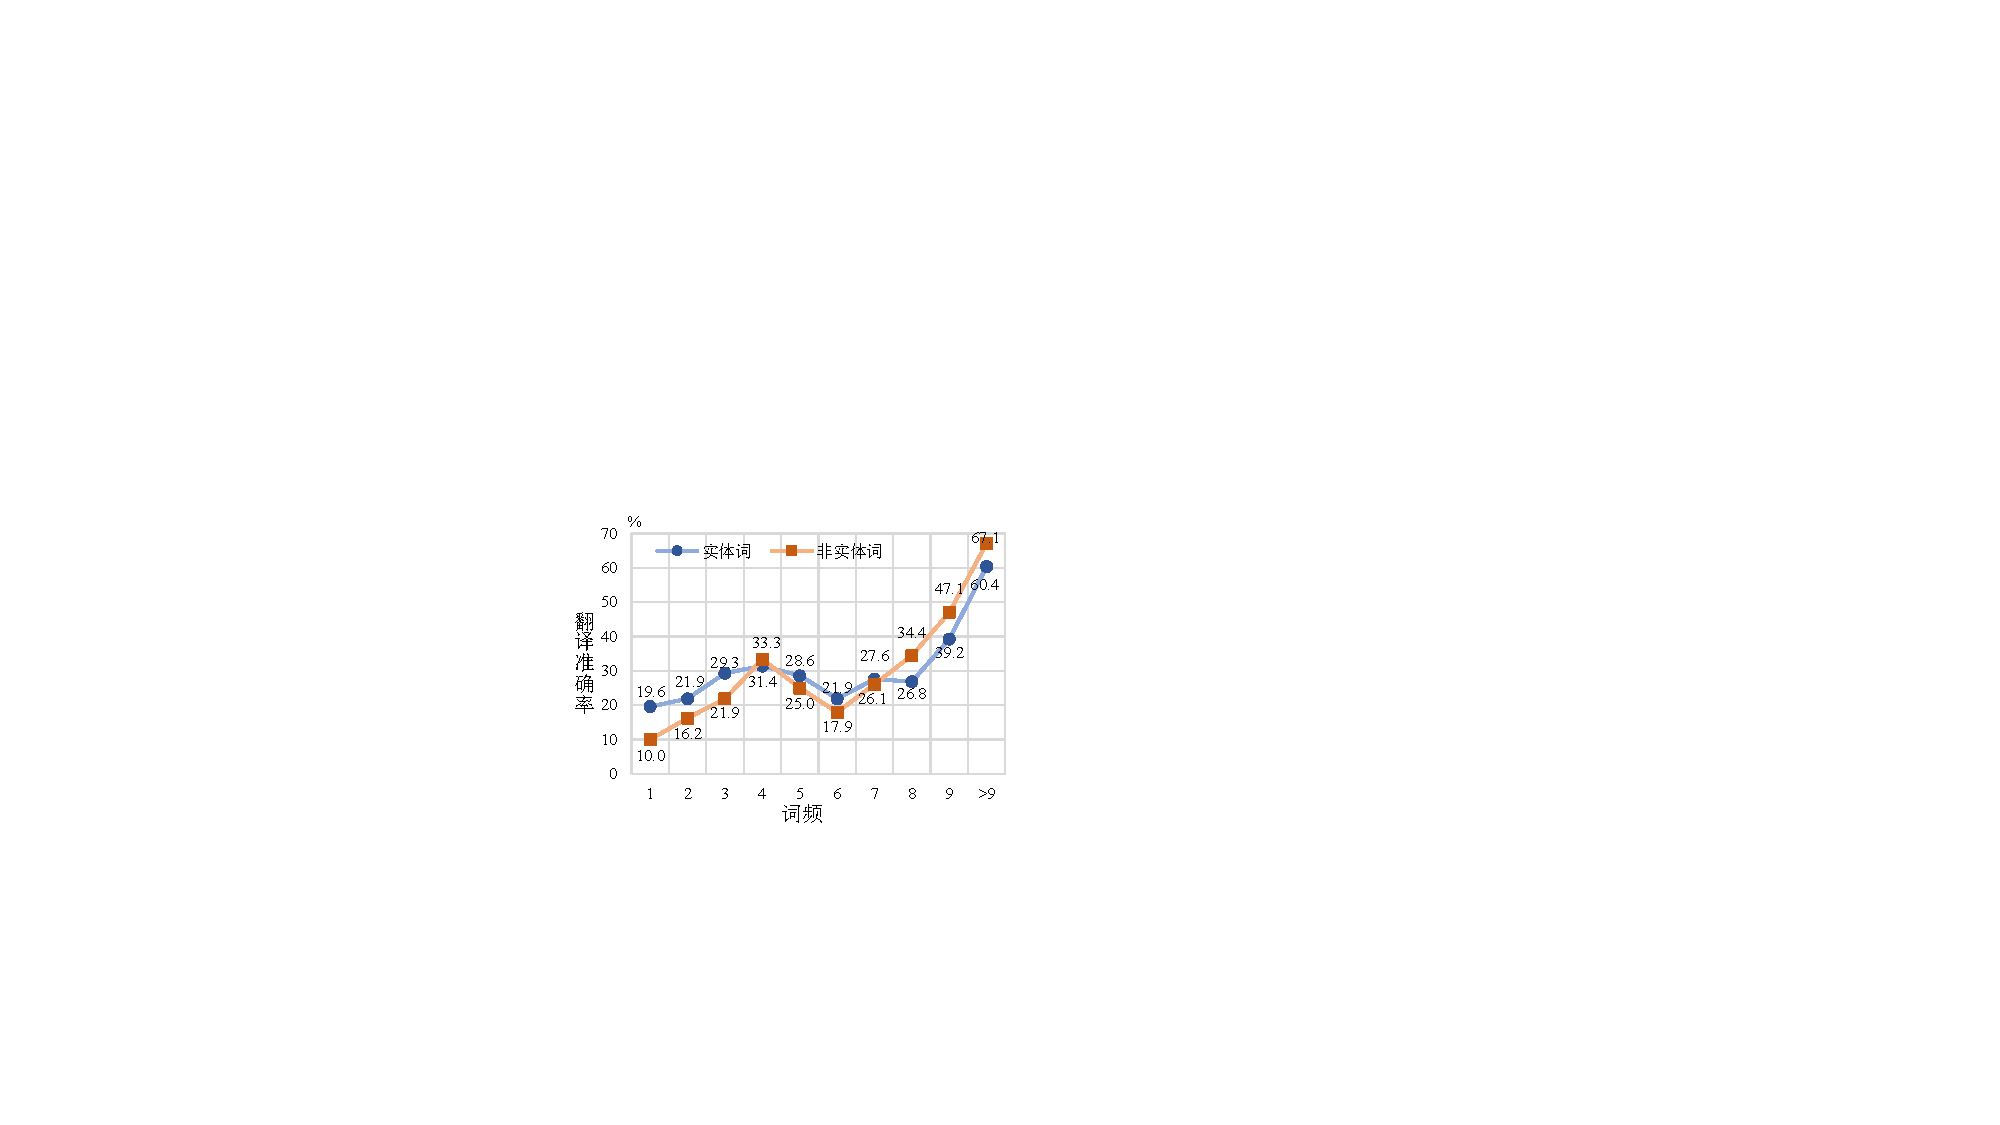
\includegraphics[width=\textwidth]{Img/fig_4_freq_acc_ctr.pdf}
      \caption{CTR-NMT}
      \label{fig:4_freq_acc_ctr}
    \end{subfigure}
    \bicaption{\centering{实体词和非实体词在不同词频下的翻译准确率}}{Translation accuracy of entity and none-entity words in different word frequencies}
    \label{fig:4_freq_acc}
\end{figure}
上一节通过统计翻译过程中目标语言的文本实体相对于源语言的文本实体的忠实度,来反映实体重构方法对翻译过程带来的影响。并发现,文本实体在翻译过程中得到了更多的重视。
为了进一步反映本章的重构方法对神经机器翻译带来的影响,我们首先统计了文本实体在所使用数据中的占比情况。统计发现,文本实体占训练集和测试集单词总数的32.6\%,文本实体在词表中的占比为59.9\%,文本实体平均词频为20.2,词频的中位数为2。根据该统计结果不难发现,大部分的实体词的词频小于等于2,反映出实体词主要分布于低频词中。这也说明了在神经机器翻译中,实体词的翻译更难。

为了探究本章的实体重构方法为文本实体的翻译带来的影响,本节统计了文本实体的翻译准确率随词频变化的统计结果。文本实体的翻译准确率的计算延续了上一节对齐原文与译文之间单词的方法。首先需要将原文与参考译文对齐进行词对齐,从而得到在每个句子中,每个单词在翻译过程中需要对齐到目标语言句子中的哪个单词。然后将神经机器翻译系统的翻译结果同样对齐到原文,从而得到该翻译系统将源语言句子中的每个词对齐到了译文中的哪个单词。通过对比所对齐的单词是否相同的方式,来判断当前单词的翻译是否正确。

图\ref{fig:4_freq_acc}展示了针对纯文本Transformer、本章的TNER-NMT、本章的CER-NMT以及上一章的CTR-NMT四个神经机器翻译系统中不同词频下的文本实体和非文本实体的翻译准确率统计情况。该统计结果基本满足随着词频的升高翻译准确率也随着升高的规律。词频较低的情况下,单词的翻译准确率的波动很大,这能够反映出模型对出现次数较少的单词的翻译置信程度较低。值得注意的是,CER-NMT和CTR-NMT都采用了明确的视觉信息作用方法,将视觉目标信息作用到文本实体上。因此这两种方法都对文本实体的翻译有较强的提升作用,这在图\ref{fig:4_freq_acc_cer}和\ref{fig:4_freq_acc_ctr}中反映在文本实体的翻译准确率在词频低于8时普遍高于文本非实体。当词频大于等于8时,虽然非实体的翻译准确率明显高于实体,但它们之间的差距明显小于Transformer和TNER-NMT的结果。


\begin{table}[!htbp]
    \bicaption{\centering{低频词与高频词的翻译准确率统计情况}}{Statistics about the translation accuracy of low-frequency words and high-frequency words}
    \label{tab:4_freq_acc}
    \centering
    \footnotesize% fontsize
    \setlength{\tabcolsep}{4pt}% column separation
    \renewcommand{\arraystretch}{1.2}%row space 
    \begin{tabular}{c|cc|cc|cc|cc}
    \hline
    %& \multicolumn{4}{c}{文本实体} & \multicolumn{4}{c}{文本非实体} \\
    %& Transformer & TNER-NMT & CER-NMT & CTER-NMT & Transformer & TNER-NMT & CER-NMT & CTER-NMT \\
    & \multicolumn{2}{c}{Transformer} & \multicolumn{2}{c}{TNER-NMT} & \multicolumn{2}{c}{CER-NMT} & \multicolumn{2}{c}{CTR-NMT} \\\cline{2-9}
      & 实体 & 非实体 & 实体 & 非实体 & 实体 & 非实体 & 实体 & 非实体 \\\hline
    低频词(<8) & 22.8 & 22.2 & 19.7 & 23.7 & 30.0 & 21.6 & 25.7 & 21.5 \\
    高频词(>=8)& 37.4 & 48.0 & 35.6 & 49.7 & 43.1 & 50.3 & 42.2 & 49.5 \\
     \hline
    \end{tabular}%
\end{table}%

图\ref{fig:4_freq_acc}反映出词频为8时,词的翻译准确率出现了一个明显的分水岭。因此,我们将词频低于8的单词作为低频词,大于等于8的为高频词,得到表\ref{tab:4_freq_acc}关于低频词和高频词的翻译准确率统计结果。从该结果中可以看出,采用显式融合方式的CER-NMT和CTR-NMT的实体词翻译准确率在低频词和高频词上均有较明显的提升,非实体词的差距并不大。CER-NMT相比于上一章的CTR-NMT有小幅度的提升,说明增加了视觉实体重构的双向实体重构方案相比于单独使用文本重构能够为实体词的翻译带来更进一步的性能提升。TNER-NMT采用了30\%的文本非实体重构,这也反映在表\ref{tab:4_freq_acc}中其低频非实体词的翻译准确率最高。

综上所述,将视觉实体明确作用到文本实体上,并进行实体级的重构方法,能够有效提升不同词频下实体词的翻译准确率,其中对低频词的提升最为明显。